%  LaTeX support: latex@mdpi.com 
%  In case you need support, please attach all files that are necessary for compiling as well as the log file, and specify the details of your LaTeX setup (which operating system and LaTeX version / tools you are using).

%=================================================================
\documentclass[sensors,article,submit,moreauthors,pdftex]{Definitions/mdpi} 
% \documentclass[preprint,article,submit,moreauthors,pdftex]{Definitions/mdpi} 

% If you would like to post an early version of this manuscript as a preprint, you may use preprint as the journal and change 'submit' to 'accept'. The document class line would be, e.g., \documentclass[preprints,article,accept,moreauthors,pdftex]{mdpi}. This is especially recommended for submission to arXiv, where line numbers should be removed before posting. For preprints.org, the editorial staff will make this change immediately prior to posting.

%--------------------
% Class Options:
%--------------------
%----------
% journal
%----------
% Choose between the following MDPI journals:
% acoustics, actuators, addictions, admsci, aerospace, agriculture, agriengineering, agronomy, algorithms, animals, antibiotics, antibodies, antioxidants, applsci, arts, asc, asi, atmosphere, atoms, axioms, batteries, bdcc, behavsci , beverages, bioengineering, biology, biomedicines, biomimetics, biomolecules, biosensors, brainsci , buildings, cancers, carbon , catalysts, cells, ceramics, challenges, chemengineering, chemistry, chemosensors, children, cleantechnol, climate, clockssleep, cmd, coatings, colloids, computation, computers, condensedmatter, cosmetics, cryptography, crystals, dairy, data, dentistry, designs , diagnostics, diseases, diversity, drones, econometrics, economies, education, ejihpe, electrochem, electronics, energies, entropy, environments, epigenomes, est, fermentation, fibers, fire, fishes, fluids, foods, forecasting, forests, fractalfract, futureinternet, futurephys, galaxies, games, gastrointestdisord, gels, genealogy, genes, geohazards, geosciences, geriatrics, hazardousmatters, healthcare, heritage, highthroughput, horticulturae, humanities, hydrology, ijerph, ijfs, ijgi, ijms, ijns, ijtpp, informatics, information, infrastructures, inorganics, insects, instruments, inventions, iot, j, jcdd, jcm, jcp, jcs, jdb, jfb, jfmk, jimaging, jintelligence, jlpea, jmmp, jmse, jnt, jof, joitmc, jpm, jrfm, jsan, land, languages, laws, life, literature, logistics, lubricants, machines, magnetochemistry, make, marinedrugs, materials, mathematics, mca, medicina, medicines, medsci, membranes, metabolites, metals, microarrays, micromachines, microorganisms, minerals, modelling, molbank, molecules, mps, mti, nanomaterials, ncrna, neuroglia, nitrogen, notspecified, nutrients, ohbm, optics, particles, pathogens, pharmaceuticals, pharmaceutics, pharmacy, philosophies, photonics, physics, plants, plasma, polymers, polysaccharides, preprints , proceedings, processes, proteomes, psych, publications, quantumrep, quaternary, qubs, reactions, recycling, religions, remotesensing, reports, resources, risks, robotics, safety, sci, scipharm, sensors, separations, sexes, signals, sinusitis, smartcities, sna, societies, socsci, soilsystems, sports, standards, stats, surfaces, surgeries, sustainability, symmetry, systems, technologies, test, toxics, toxins, tropicalmed, universe, urbansci, vaccines, vehicles, vetsci, vibration, viruses, vision, water, wem, wevj

%---------
% article
%---------
% The default type of manuscript is "article", but can be replaced by: 
% abstract, addendum, article, benchmark, book, bookreview, briefreport, casereport, changes, comment, commentary, communication, conceptpaper, conferenceproceedings, correction, conferencereport, expressionofconcern, extendedabstract, meetingreport, creative, datadescriptor, discussion, editorial, essay, erratum, hypothesis, interestingimages, letter, meetingreport, newbookreceived, obituary, opinion, projectreport, reply, retraction, review, perspective, protocol, shortnote, supfile, technicalnote, viewpoint
% supfile = supplementary materials

%----------
% submit
%----------
% The class option "submit" will be changed to "accept" by the Editorial Office when the paper is accepted. This will only make changes to the frontpage (e.g., the logo of the journal will get visible), the headings, and the copyright information. Also, line numbering will be removed. Journal info and pagination for accepted papers will also be assigned by the Editorial Office.

%------------------
% moreauthors
%------------------
% If there is only one author the class option oneauthor should be used. Otherwise use the class option moreauthors.

%---------
% pdftex
%---------
% The option pdftex is for use with pdfLaTeX. If eps figures are used, remove the option pdftex and use LaTeX and dvi2pdf.

%=================================================================
\firstpage{1} 
\makeatletter 
\setcounter{page}{\@firstpage} 
\makeatother
\pubvolume{xx}
\issuenum{1}
\articlenumber{5}
\pubyear{2019}
\copyrightyear{2019}
%\externaleditor{Academic Editor: name}
\history{Received: date; Accepted: date; Published: date}
%\updates{yes} % If there is an update available, un-comment this line

%% MDPI internal command: uncomment if new journal that already uses continuous page numbers 
%\continuouspages{yes}

%------------------------------------------------------------------
% The following line should be uncommented if the LaTeX file is uploaded to arXiv.org
%\pdfoutput=1

%=================================================================
% Add packages and commands here. The following packages are loaded in our class file: fontenc, calc, indentfirst, fancyhdr, graphicx, lastpage, ifthen, lineno, float, amsmath, setspace, enumitem, mathpazo, booktabs, titlesec, etoolbox, amsthm, hyphenat, natbib, hyperref, footmisc, geometry, caption, url, mdframed, tabto, soul, multirow, microtype, tikz
\usepackage{caption}
\usepackage{subcaption}
%=================================================================
%% Please use the following mathematics environments: Theorem, Lemma, Corollary, Proposition, Characterization, Property, Problem, Example, ExamplesandDefinitions, Hypothesis, Remark, Definition, Notation, Assumption
%% For proofs, please use the proof environment (the amsthm package is loaded by the MDPI class).

%=================================================================
% Full title of the paper (Capitalized)
\Title{Untitled Article}

% Author Orchid ID: enter ID or remove command
\newcommand{\orcidauthorA}{0000-0003-3611-4846} % Add \orcidA{} behind the author's name
\newcommand{\orcidauthorB}{0000-0002-4965-0341} % Add \orcidB{} behind the author's name

% Authors, for the paper (add full first names)
\Author{Frederick Sherratt $^{1,\dagger,\ddagger}$\orcidA{} and Pejman Iravani $^{2,}$*\orcidB{}}

% Authors, for metadata in PDF
\AuthorNames{Frederick Sherratt and Pejman Iravani}

% Affiliations / Addresses (Add [1] after \address if there is only one affiliation.)
\address{%
$^{1}$ \quad Affiliation 1; e-mail@e-mail.com\\
$^{2}$ \quad Affiliation 2; e-mail@e-mail.com}

% Contact information of the corresponding author
\corres{Correspondence: e-mail@e-mail.com; Tel.: (optional; include country code; if there are multiple corresponding authors, add author initials) +xx-xxxx-xxx-xxxx (F.L.)}

% Current address and/or shared authorship
\firstnote{Current address: Affiliation 3} 
\secondnote{These authors contributed equally to this work.}
% The commands \thirdnote{} till \eighthnote{} are available for further notes

%\simplesumm{} % Simple summary

%\conference{} % An extended version of a conference paper

% Abstract (Do not insert blank lines, i.e. \\) 
\abstract{ }
% \abstract{A single paragraph of about 200 words maximum. For research articles, abstracts should give a pertinent overview of the work. We strongly encourage authors to use the following style of structured abstracts, but without headings: (1) Background: Place the question addressed in a broad context and highlight the purpose of the study; (2) Methods: Describe briefly the main methods or treatments applied; (3) Results: Summarize the article's main findings; and (4) Conclusion: Indicate the main conclusions or interpretations. The abstract should be an objective representation of the article, it must not contain results which are not presented and substantiated in the main text and should not exaggerate the main conclusions.}

% Keywords
\keyword{ }
% \keyword{keyword 1; keyword 2; keyword 3 (list three to ten pertinent keywords specific to the article, yet reasonably common within the subject discipline.)}

% The fields PACS, MSC, and JEL may be left empty or commented out if not applicable
%\PACS{J0101}
%\MSC{}
%\JEL{}

%%%%%%%%%%%%%%%%%%%%%%%%%%%%%%%%%%%%%%%%%%
% Only for the journal Diversity
%\LSID{\url{http://}}

%%%%%%%%%%%%%%%%%%%%%%%%%%%%%%%%%%%%%%%%%%
% Only for the journal Applied Sciences:
%\featuredapplication{Authors are encouraged to provide a concise description of the specific application or a potential application of the work. This section is not mandatory.}
%%%%%%%%%%%%%%%%%%%%%%%%%%%%%%%%%%%%%%%%%%

%%%%%%%%%%%%%%%%%%%%%%%%%%%%%%%%%%%%%%%%%%
% Only for the journal Data:
%\dataset{DOI number or link to the deposited data set in cases where the data set is published or set to be published separately. If the data set is submitted and will be published as a supplement to this paper in the journal Data, this field will be filled by the editors of the journal. In this case, please make sure to submit the data set as a supplement when entering your manuscript into our manuscript editorial system.}

%\datasetlicense{license under which the data set is made available (CC0, CC-BY, CC-BY-SA, CC-BY-NC, etc.)}

%%%%%%%%%%%%%%%%%%%%%%%%%%%%%%%%%%%%%%%%%%
% Only for the journal Toxins
%\keycontribution{The breakthroughs or highlights of the manuscript. Authors can write one or two sentences to describe the most important part of the paper.}

%\setcounter{secnumdepth}{4}
%%%%%%%%%%%%%%%%%%%%%%%%%%%%%%%%%%%%%%%%%%
\begin{document}
%%%%%%%%%%%%%%%%%%%%%%%%%%%%%%%%%%%%%%%%%%

%%%%%%%%%%%%%%%%%%%%%%%%%%%%%%%%%%%%%%%%%%
\section{Introduction}
%purpose/uses of HAR
Human Activity Recognition systems have numerous health applications, such as monitoring of physical activity level to manage health conditions or automatic gait mode selection of lower limb prosthesis. Classification accuracy is the key factor in determining the performance of these systems, along with generalization i.e. their flexibility of the classifier to support new users.\cite{Ponce2016}

%Background - % What activities, sensors, Feature selection, performance has been achieved
Non-invasive wearable sensors, such as Inertial Measurement Units, are an appealing choice for developing such a system. 
% Something about heuristics
The current state of the art activity recognition papers using IMUs uses Long Short Term Network LSTM base Machine Learning ML techniques to achieve high levels of classification. These have been shown to achieve 95\%\cite{Murad2017} accuracy.

% Problems\Research gaps
Dehghani et al investigate the metrics used to evaluate the performance of classifiers in regard to there performance to previously unseen data presented using k-fold cross-validation methods\cite{Dehghani2019}. The papers found implement various forms of k-fold validation but none using LSTM use a subject based cross-validation. Instead, they either leave out individual windows \cite{Murad2017, Wang2020}<TK> or, when multiple data sets are recorded for participants, individual recordings \cite{Ordonez2016}<TK>. Dehghani found that this overestimates performance by 10-16\%. Studies that have left individuals out found accuracies closer of 86.7\% \cite{Zhao2018}. The reason for the poor generalisation when presented with a novel user has not been investigated.

In this paper, we train simplified LSTM networks to classify simplified HAR problems. These models are then analysed in detail to understand their operation. The learning from this is then applied to more complicated networks to demonstrate this learning can be applied more generally. The major contributions of this work are as follows:
\begin{enumerate}
\item Lorem ipsum dolor sit amet
\item Consectetur adipiscing elit
\end{enumerate}

The remainder of this paper is organized as follows;

\subsection{Related Works}
% Related works - What have people tried so far in terms of generalisation


\section{Background}
%LSTM theory of operation
\subsection{LSTM Operation}
The Long Short Term network was created as a solution to the vanishing/exploding gradient problem found in Stock Recursive Neural Networks (RNN). The LSTM allows training gradients to flow for long duration's preventing them tending to extreme values. The LSTM cell contains a system of parameters and gaiting that controls the flow of information that allow it to be retained or forgotten. Like a standard RNN information may only move forward in time through an LSTM cell but can mix in other dimensions freely, i.e. the LSTM network cell inputs/outputs are fully connected between time steps.

%MARG HAR Data
\subsection{Gait Cycle}

%%%%%%%%%%%%%%%%%%%%%%%%%%%%%%%%%%%%%%%%%%
\section{Methodology}
The following section describes the methodology used to investigate the proposed research question.

\subsection{Data Collection}
% Existing data sets?
A wearable IMU produced by Movesense was used to collect activity data. This sensor contains a 9 axis MARG (Magnetic, Angular Rate and Gravity) in and a Bluetooth radio powered by a coin cell battery. The sensor housing contains a snap connectors allowing it to be clipped into attachment hardware and a variety of mounting hardware is available off the shelf. The sensor is user-programmable allowing customised behaviour. For this study, the sensor was programmed to form a Bluetooth Low Energy (BLE) connection and broadcast 100Hz MARG sensors data. % Explain sensor selection

5 sensors were attached to each participant, an the inside of ankle using an elastic Velcro strap, each hip using a clothes/belt clip and the chest using a heart rate strap. These provided secure non-invasive attachment to minimise discomfort and disruption of natural movement. The data from each sensor was live-streamed recorded at 100Hz to a custom android app. For this investigation, only the ankle data will be used. The app contained buttons for real-time annotation of the data. 

Twenty-two Participants of a wide variety of age, gender and physique were chosen to give a broad data set. Participants were instructed to walk around a varied environment with the sensor on, and label their activity as they went. Participants were asked to label the following activities; Walking (W), Stair Ascent (SA), Stair Descent (SD), Ramp Ascent (RA) and Ramp Descent (RD). No further instructions on how the activities should be conducted were provided. This produced a unique self-supervised set of IMU activity data. The self-supervised nature has provided data from a wide range of environments being collected with participants moving at there natural walking speeds with no influence for the researchers.

To convert the raw saved data to a form that Tensorflow could understand from using a processing pipeline was developed in Matlab 2019b. The pipeline consisted of decoding, re-sampling, normalisation, and saving. The data is saved raw from the sensor so needed to be converted from compressed hexadecimal fixed point form to a floating-point representation. The data was then re-sampled to compensate for the difference between the internal sensor clock, the android smartphone clock was used as a common reference for this adjustment. The data was normalised so that for each recording every individual sensor channel had a standard deviation of one and a mean of zero.

\subsection{Training}
The adam optimisation algorithm was used, a popular algorithm for problems with large data-sets and or parameters[1]. The training was undertaken using GPU acceleration with models defined using the Keras Tensorflow 2.1.0 language. Initial model weights were set using a Golorot Uniform initialiser. A class weight input was used to bias the training as a balance for in-balanced data labels.

A sliding data window with an offset of 2 samples between them. The offset was set empirically to give the model a wide range of data from any window position without slowing down training from an unnecessarily large data set. The label for each widow was set as the recorded ground truth at the end of the window, these are provided to the network in a one-hot encoding. 

The training data set is divided into two groups a test and training. Test contains 5 participants to be excluded from the training process. The test set is used to access the performance of the models to unseen data novel participants. The training set contains the remaining participants. The training set was reduced so that no label class contains more than 50\% greater labels than any another. For each model, the training data 30\% was retained as validation the remaining 70\% used for training. The data was split randomly but care was taken to ensure the balance of each label type was maintained.

% Analysis methods

%%%%%%%%%%%%%%%%%%%%%%%%%%%%%%%%%%%%%%%%%%
\section{Results}
% Define axis

\subsection{Individual Gait Trends}
\begin{figure}[!htb]
     \centering
     \begin{subfigure}[b]{0.49\textwidth}
         \centering
         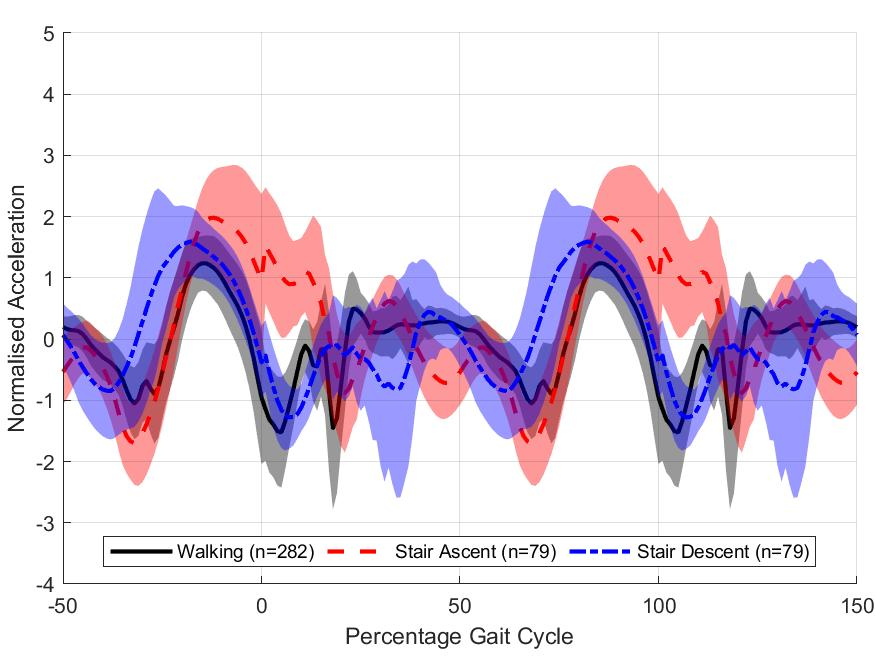
\includegraphics[width=\textwidth]{Figures/accel_x_trend_Participant_04.jpg}
         \caption{Subject 4 - Acceleration in x}
         \label{fig:x_accel_subj_4}
     \end{subfigure}
     \hfill
     \begin{subfigure}[b]{0.49\textwidth}
         \centering
         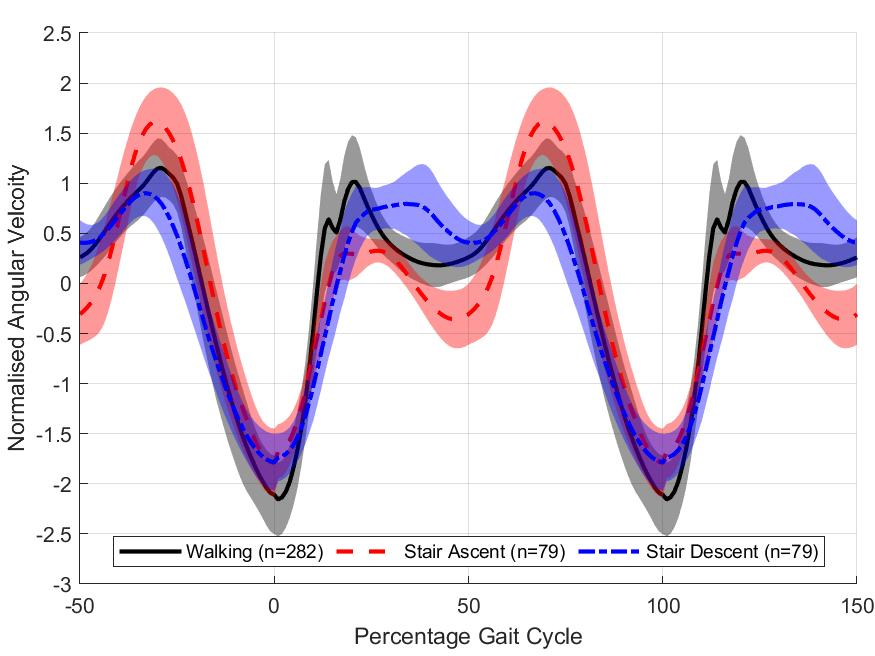
\includegraphics[width=\textwidth]{Figures/gyro_y_trend_Participant_04.jpg}
         \caption{Participant 4 - Angular velocity about y}
         \label{fig:x_gyro_subj_4}
     \end{subfigure}
     \vskip\baselineskip
     \begin{subfigure}[b]{0.49\textwidth}
         \centering
         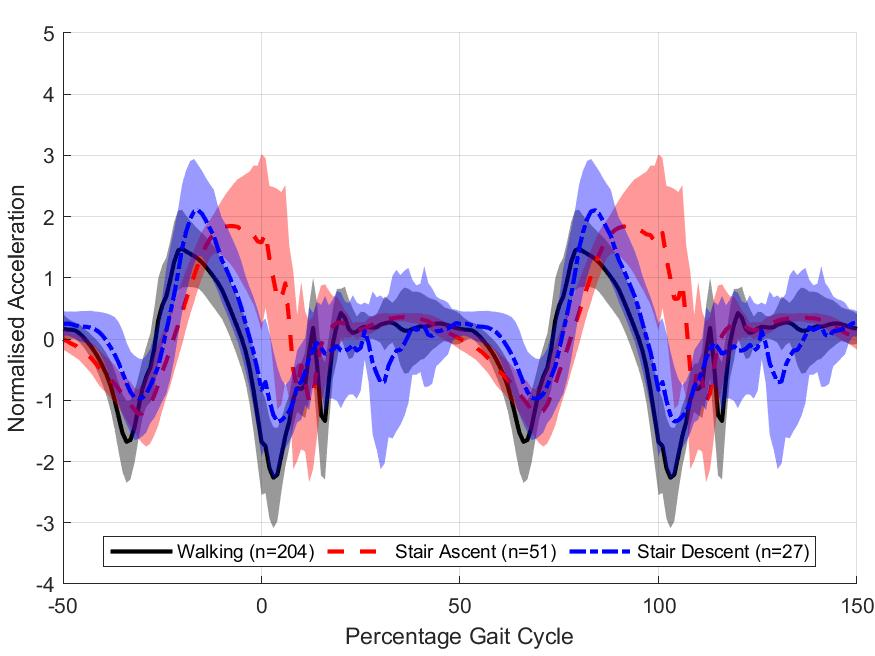
\includegraphics[width=\textwidth]{Figures/accel_x_trend_Participant_16.jpg}
         \caption{Subject 16 - Acceleration in x}
         \label{fig:x_accel_subj_16}
     \end{subfigure}
     \hfill
     \begin{subfigure}[b]{0.49\textwidth}
         \centering
         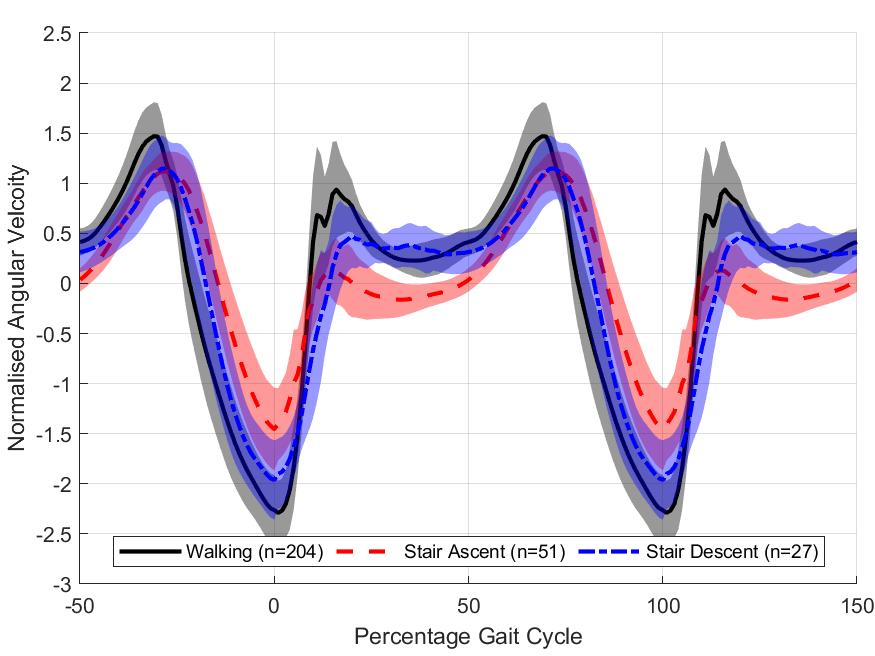
\includegraphics[width=\textwidth]{Figures/gyro_y_trend_Participant_16.jpg}
         \caption{Participant 16 - Angular velocity about y}
         \label{fig:x_gyro_subj_16}
     \end{subfigure}
    \caption{Examples of gait trends of two subject for 3 different activities. The solid lines show the mean value for n steps, the shaded area shows the standard deviation}
    \label{fig:imu_gait_trends}
\end{figure}

%%%%%%%%%%%%%%%%%%%%%%%%%%%%%%%%%%%%%%%%%%

%%%%%%%%%%%%%%%%%%%%%%%%%%%%%%%%%%%%%%%%%%
\section{Discussion}

%%%%%%%%%%%%%%%%%%%%%%%%%%%%%%%%%%%%%%%%%%
\section{Conclusions}

%%%%%%%%%%%%%%%%%%%%%%%%%%%%%%%%%%%%%%%%%%
\vspace{6pt} 

%%%%%%%%%%%%%%%%%%%%%%%%%%%%%%%%%%%%%%%%%%
%% optional
%\supplementary{The following are available online at \linksupplementary{s1}, Figure S1: title, Table S1: title, Video S1: title.}

% Only for the journal Methods and Protocols:
% If you wish to submit a video article, please do so with any other supplementary material.
% \supplementary{The following are available at \linksupplementary{s1}, Figure S1: title, Table S1: title, Video S1: title. A supporting video article is available at doi: link.}

%%%%%%%%%%%%%%%%%%%%%%%%%%%%%%%%%%%%%%%%%%
\authorcontributions{For research articles with several authors, a short paragraph specifying their individual contributions must be provided. The following statements should be used ``conceptualization, X.X. and Y.Y.; methodology, X.X.; software, X.X.; validation, X.X., Y.Y. and Z.Z.; formal analysis, X.X.; investigation, X.X.; resources, X.X.; data curation, X.X.; writing--original draft preparation, X.X.; writing--review and editing, X.X.; visualization, X.X.; supervision, X.X.; project administration, X.X.; funding acquisition, Y.Y.'', please turn to the  \href{http://img.mdpi.org/data/contributor-role-instruction.pdf}{CRediT taxonomy} for the term explanation. Authorship must be limited to those who have contributed substantially to the work reported.}

%%%%%%%%%%%%%%%%%%%%%%%%%%%%%%%%%%%%%%%%%%
\funding{Please add: ``This research received no external funding'' or ``This research was funded by NAME OF FUNDER grant number XXX.'' and  and ``The APC was funded by XXX''. Check carefully that the details given are accurate and use the standard spelling of funding agency names at \url{https://search.crossref.org/funding}, any errors may affect your future funding.}

%%%%%%%%%%%%%%%%%%%%%%%%%%%%%%%%%%%%%%%%%%
\acknowledgments{In this section you can acknowledge any support given which is not covered by the author contribution or funding sections. This may include administrative and technical support, or donations in kind (e.g., materials used for experiments).}

%%%%%%%%%%%%%%%%%%%%%%%%%%%%%%%%%%%%%%%%%%
\conflictsofinterest{The authors declare no conflict of interest. The funders had no role in the design of the study; in the collection, analyses, or interpretation of data; in the writing of the manuscript, or in the decision to publish the results.} 

%%%%%%%%%%%%%%%%%%%%%%%%%%%%%%%%%%%%%%%%%%
%% optional
\abbreviations{The following abbreviations are used in this manuscript:\\

\noindent 
\begin{tabular}{@{}ll}
HAR & Human Activity Recognition\\
ML & Machine Learning\\
LSTM & Long Short Term Memory\\
RNN & Recurrent Neural Network\\
\end{tabular}}

%%%%%%%%%%%%%%%%%%%%%%%%%%%%%%%%%%%%%%%%%%
%% optional
%%%%%%%%%%%%%%%%%%%%%%%%%%%%%%%%%%%%%%%%%%
% Citations and References in Supplementary files are permitted provided that they also appear in the reference list here. 

%=====================================
% References, variant A: internal bibliography
%=====================================
\reftitle{References}
% \begin{thebibliography}{999}
% % Reference 1
% \bibitem[Author1(year)]{ref-journal}
% Author1, T. The title of the cited article. {\em Journal Abbreviation} {\bf 2008}, {\em 10}, 142--149.
% % Reference 2
% \bibitem[Author2(year)]{ref-book}
% Author2, L. The title of the cited contribution. In {\em The Book Title}; Editor1, F., Editor2, A., Eds.; Publishing House: City, Country, 2007; pp. 32--58.
% \end{thebibliography}

% The following MDPI journals use author-date citation: Arts, Econometrics, Economies, Genealogy, Humanities, IJFS, JRFM, Laws, Religions, Risks, Social Sciences. For those journals, please follow the formatting guidelines on http://www.mdpi.com/authors/references
% To cite two works by the same author: \citeauthor{ref-journal-1a} (\citeyear{ref-journal-1a}, \citeyear{ref-journal-1b}). This produces: Whittaker (1967, 1975)
% To cite two works by the same author with specific pages: \citeauthor{ref-journal-3a} (\citeyear{ref-journal-3a}, p. 328; \citeyear{ref-journal-3b}, p.475). This produces: Wong (1999, p. 328; 2000, p. 475)

%=====================================
% References, variant B: external bibliography
%=====================================
\externalbibliography{yes}
\bibliography{references}

%%%%%%%%%%%%%%%%%%%%%%%%%%%%%%%%%%%%%%%%%%
%% optional
%% for journal Sci
%\reviewreports{\\
%Reviewer 1 comments and authors’ response\\
%Reviewer 2 comments and authors’ response\\
%Reviewer 3 comments and authors’ response
%}

%%%%%%%%%%%%%%%%%%%%%%%%%%%%%%%%%%%%%%%%%%
\end{document}

